% cd.tex

\documentclass[11pt,oneslide,a4paper,titlepage]{article}

\usepackage[most]{tcolorbox}
\usepackage{geometry}

\usepackage{geometry}
\geometry{
	a4paper,
	left=0.1cm,
	right=0.1cm,
	top=0.1cm,
	bottom=0.1cm
}

\definecolor{titleBack}{RGB}{0, 104, 157}

\title{QuantitativeBytes}
\date{}

\begin{document}
\tcbset{colframe=gray!95!black,colback=titleBack,arc=0mm}

\begin{tcolorbox}
	\begin{minipage}{4.5cm}
		\hspace*{0.3cm}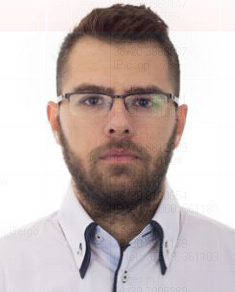
\includegraphics[width=3.6cm]{pictures/pic.png}
	\end{minipage}
	\begin{minipage}{15cm}
		\begin{center}
			\Huge{\textcolor{white}{István Nagy}} \\
			\vspace*{0.5cm}
			\Large{\textcolor{white}{{Electrical Engineer - Embedded Systems}}}
		\end{center}
	\end{minipage}
\end{tcolorbox}

\tcbset{colframe=white,colback=white,arc=0mm}
\begin{tcolorbox}
	\begin{minipage}[t]{8cm}
		\vspace*{-0.5cm}
		\begin{tcolorbox}[grow to left by=0.6cm,colback=gray!25,colframe=white]
			\section*{Profile}
			Passionate about programming and learning new technologies. I have gathered experiences as software developer mostly in the field of Automotive and Automation Systems. From both fields I have learnt how to make reliable and safe software and hardware components. \newline
			I have developed projects started from making specifications and requirements through making software and hardware component to documentation and delivery. \newline
			I like to work indepedently but also I consider myself as a team player especially when a project requires other engineering fields to be merged.

			\section*{Contact}
			Address: 2120 Dunakeszi Petőfi utca 13. \\
			Phone: +36 30 833 6719 \\
			Email: istvan.nagy1995@live.com \\
			LinkedIn: istvan-nagy-98baa3122 \\

			\section*{Expertise}
			\begin{itemize}
				\item{C/C++, Python, Latex, PCB design}
				\item{Image processing, Computer Vision}
				\item{AUTOSAR Classic Platform, Git}
				\item{FreeRTOS, Linux, STM32, Raspberry Pi}
			\end{itemize}
			
			\section*{Languages}
			\begin{itemize}
				\item{English(B2) - Daily use and professional working proficiency}
				\item{Hungarian - Native}
			\end{itemize}
			
			\section*{Other interests}
			\begin{itemize}
				\item{Music production - FLStudio}
				\item{VJ production - Resolume	}
			\end{itemize}													
		\end{tcolorbox}
	\end{minipage}
	\begin{minipage}[t]{11cm}
		\vspace*{-0.5cm}
		\begin{tcolorbox}[grow to right by=0.75cm,colframe=white,colback=white]
			\section*{Education}
			\begin{itemize}
				\item{
					\textbf{Óbuda University - KVK} \\
					\emph{Electrical Engineer (BSc.)} \\
					\emph{2015 - 2019} \\
					\emph{Specialisation: Automation - Embedded Systems expert} \\
					\emph{Classification of the qualification: Outstanding}
				}
			\end{itemize}
			\section*{Experiences}
			\begin{itemize}
				\item{
					\textbf{Electronics Development Engineer} \\	
					\emph{Unix Autó Kft. (2021 - Present)} \\
					\newline I was the part of the Research and Development team. The main portfolio of the department was warehouse automation system development. \\
					\newline \underline{I was responsible for:}
					\begin{itemize}
						\item{specificate and making requirements about the project and calculate deadlines for each individual tasks}
						\item{design circuit in Altium or KiCAD with 2 or 4 layers of PCB (THT and SMD components as well)}
						\item{search and order required components and keeping contact with suppliers}
						\item{developing source code for STM32 development boards (or Raspberry Pi)}
						\item{Making unit test framework for functional testing and lifetime testing hardware components}
						\item{Prepare user guide or assembly guide for technicians (with Latex and UML)}
					\end{itemize}
					
					\hfill\break
					\textbf{Few of my projects:} \\
				    \newline \textbf{Robot arm positioning with computer vision:} I was developing QR Code detection algorithm with the help of OpenCV in C++. The QR code was responsible to show the middle point of an object. If the center point was found then the coordinates were sent via CAN to a STM32 control board and the robot arm was moving according to that. \\
				}
			\end{itemize}				
			
		\end{tcolorbox}
	\end{minipage}
\end{tcolorbox}

\newpage
\tcbset{colframe=white,colback=white,arc=0mm}
\begin{tcolorbox}
	\begin{minipage}[t]{8cm}
		\vspace*{-0.5cm}
		\begin{tcolorbox}[grow to left by=0.6cm,colback=gray!25,colframe=white]
			\vspace*{0.5cm}
			\section*{Design softwares}
			\hfill\break
			STM32CubeIDE, Visual Studio Code, Altium, KiCAD, FreeCAD, 					Eclipse IDE, TexMaker, GitExtension	
			\section*{Soft skills}
		    Critical thinker, Good problem solving, Attentive listening and effective oral communication, good leadership skills, fast learner				
		\end{tcolorbox}
	\end{minipage}
	\begin{minipage}[t]{11cm}
		\vspace*{0.5cm}
		\begin{tcolorbox}[grow to right by=0.75cm,colframe=white,colback=white]
			\begin{itemize}
			\item[]{
				\textbf{Slide level detection with computer vision:} The task was to check how full are the slides with boxes. I trained a YOLO AI modell to detect boxes but because of the lack of the computation power i redesigned and finalized the project with contour detection. \\ 

				\textbf{Robot motion control source code generator:}
I developed a source code generator for robot control in Python with the help of Jinja2.
A few source code template were created and with the help of them a complete robot motion sequence could be generated instead of writting couple thousand lines of code.
			}
			\end{itemize}
			
			\hfill\break
			\begin{itemize}
				\item{
					\textbf{Embedded Software Development Engineer} \\
					\emph{Siemens EDA Kft., (Mentor Graphics Kft.) (2019 - 2021)} \\
						\hfill\break
	   				    I was developing and maintaning AUTOSAR modules which were part of the Classis Platform. Most modules were inside \textbf{"Basic Software"} software layer. \\
						\hfill\break
	    				BSW modules I have experiences: NvM, Ea, MemIf, Crc, KeyM, Fr(If,Tp,Nm,SM), Dem, Dlt, Wdg(If,M), Can(If,Nm,SM) \\
						\hfill\break
						\underline{Development included:}
						\begin{itemize}
							\item{
								source code writing according to SWS (in C language)		
							}
							\item{
								develop configuration generator (in Java language)
							}
							\item{
								make configuration for each module (in ARXML format)
							}
							\item{
								writing unit tests and check code coverage with the help of Bullseye	
							}
							\item{
								making User Guide and Software Design Guide (in LATEX and UML format)			
							}
						\end{itemize}
		
				Development strictly followed ISO26262 (from ASIL A to D) and Automotive SPICE. Jira was used for project management tool.
				}
				\hfill\break
				\item{
					\textbf{Electrical Technician (Intern during university)} \\
					\emph{Eco Cranes Kft. (2017-2018)}
					\begin{itemize}
						\item{Power supply implementation for cranes}
						\item{Remote control configuration and wiring}
						\item{Different crane service tasks}
					\end{itemize}
				}
			\end{itemize}
			
		\end{tcolorbox}
	\end{minipage}
\end{tcolorbox}


\end{document}
